\documentclass[10pt,letterpaper]{article}
\usepackage[utf8]{inputenc}
\usepackage{amsmath}
\usepackage{amsfonts}
\usepackage{amssymb}
\usepackage{graphicx}
\usepackage{subcaption}

\author{Daniil Bochkov}
\title{Solving 0D Boltzmann equation using Maxwell polynomials and spherical harmonics}

\newcommand{\myint}[2]{\int\limits_{#1}^{#2}}
\newcommand{\diff}[1]{\, d#1}
\newcommand{\vect}[1]{\mathbf{#1}}
\usepackage{mleftright}
\newcommand{\of}[1]{\mleft( #1 \mright)}
\newcommand{\ddt}[1]{\partial_t #1}
\newcommand{\vth}{v_\textrm{th}}
\newcommand{\reals}{\mathbb{R}}

\begin{document}
\section*{Solving homogeneous Boltzmann equation in spherical coordinates}
Let us denote the velocity vector as $\vect{v}$ and its magnitude as $v$. In the spatially homogeneous case of collisions between electrons and immobile (infinitely heavy) neutrals the Boltzmann equation takes the form 
\begin{align*}
\ddt{f}\of{\vect{v},t} = 
\myint{S^2}{}
B\of{v,\omega} \left( f\of{\vect{v}^\prime, t} - f\of{\vect{v},t} \right) \diff{\omega}
\end{align*}
Projecting the equation onto a test function $\phi\of{\vect{v}}$ gives the following variational formulation
\begin{align*}
\ddt{} \myint{\reals^3}{} f\of{\vect{v},t} \phi\of{\vect{v}} \diff{\vect{v}} =
\myint{\reals^3}{} 
\myint{S^2}{}
B\of{v,\omega} \left( f\of{\vect{v}^\prime, t} - f\of{\vect{v},t} \right) \phi\of{\vect{v}} \diff{\omega}
\diff{\vect{v}} 
\end{align*}
Assume $f\of{\vect{v}}$ deviates from the Maxwell-Boltzmann velocity distribution\footnote{Not sure what's the right thing to call it, but this is essentially a three-dimensional Gaussian distribution and should not be confused with the Maxwell-Boltzmann distribution which describes distribution for speed and $\sim v^2 e^{-\frac{v}{\vth}}$} only slightly
\begin{align*}
f\of{\vect{v}} = M\of{v} \left( 1 + h\of{\vect{v},t} \right)
\end{align*}
where $M\of{v}$ denotes
\begin{align*}
M\of{v} = \frac{n}{\left( \vth \sqrt{\pi} \right)^3} e^{-\left(\frac{v}{\vth}\right)^2}
\end{align*}
This leads to
\begin{align*}
\myint{\reals^3}{} M\of{v} \ddt{} h\of{\vect{v},t} \phi\of{\vect{v}} \diff{\vect{v}} &=
\myint{\reals^3}{} 
\myint{S^2}{}
B\of{v,\omega} \left( M\of{v^\prime} - M\of{v} \right) \phi\of{\vect{v}} \diff{\omega}
\diff{\vect{v}} 
\\
&+
\myint{\reals^3}{} 
\myint{S^2}{}
B\of{v,\omega} \left( M\of{v^\prime} h\of{\vect{v}^\prime, t} - M\of{v} h\of{\vect{v},t} \right) \phi\of{\vect{v}} \diff{\omega}
\diff{\vect{v}} 
\end{align*}

One option is to approximate $h\of{\vect{v}, t}$ in Cartesian coordinates using Hermite polynomials
\begin{align*}
h\of{\vect{v},t} \approx
\sum_{i,j,k} h_{i,j,k} \of{t} P_i\of{\frac{v_x}{\vth}} P_j\of{\frac{v_y}{\vth}}  P_k\of{\frac{v_z}{\vth}} 
\end{align*}
which satisfy the property
\begin{align*}
\myint{-\infty}{+\infty} e^{-x^2} P_i\of{x} P_{i^\prime}\of{x} \diff{x} \sim \delta_{ii^\prime}
\end{align*}
Here another option is summarized: approximate $h\of{\vect{v}, t}$ in spherical coordinates using a combination of real-valued spherical harmonics with either the so-called ``Maxwell'' polynomials or the more traditional associated Laguerre polynomials
\begin{align*}
h\of{\vect{v},t} &\approx
\sum_{k,l,m} h_{k,l,m} \of{t} P_k\of{\frac{v}{\vth}} Y_{lm}\of{v_\theta, v_\phi}
\\
h\of{\vect{v},t} &\approx
\sum_{k,l,m} h_{k,l,m} \of{t} L_k\of{\frac{v^2}{\vth^2}} Y_{lm}\of{v_\theta, v_\phi}
\end{align*}
Let us define the ``Maxwell'' polynomials as 
\begin{align*}
\myint{0}{+\infty} \frac{4}{\sqrt{\pi}} x^2 e^{-x^2} P_k\of{x} P_{k^\prime}\of{x} \diff{x} = \delta_{kk^\prime}
\end{align*}
and the associated Laguerre polynomials as
\begin{align*}
\myint{0}{+\infty} \frac{4}{\sqrt{\pi}} x^2 e^{-x^2} L_k\of{x^2} L_{k^\prime}\of{x^2} \diff{x} &= \delta_{kk^\prime}
\end{align*}
or, equivalently, 
\begin{align*}
\myint{0}{+\infty} \frac{2}{\sqrt{\pi}} \sqrt{y} e^{-y} L_k\of{y} L_{k^\prime}\of{y} \diff{y} &= \delta_{kk^\prime}
\end{align*}
Such polynomials can be generated (up to the normalization constant) by the following recursive relation
\begin{align*}
P_{-1}\of{x} &= 0, \\
P_{0}\of{x} &= 1, \\
P_{n+1}\of{x} &= (x-a_n) P_{n}\of{x} - b_n P_{n-1} \of{x},
\end{align*}
where
\begin{align*}
a_n = \frac{\left< x P_n, P_n \right>}{\left< P_n, P_n \right>}, \quad
b_n = \frac{\left< P_n, P_n \right>}{\left< P_{n-1}, P_{n-1} \right>}, \quad
\left< f, g \right> = \myint{0}{\infty} f\of{x} g\of{x} \frac{4}{\sqrt{\pi}} x^2 e^{-x^2} \diff{x}
\end{align*}
(If only first several polynomials are needed we could probably just generated them analytically in Mathematica. I wrote a short script for that if needed.)

A few first of such polynomials are given by
\begin{align*}
P_0\of{x} & = 1,
\\
P_1\of{x} & = \sqrt{\frac{2 \pi }{3 \pi -8}} x-2 \sqrt{\frac{2}{3 \pi -8}},
\\
P_2\of{x} & = \frac{6 \pi  \sqrt{2} x^2-16 \sqrt{2} x^2-4 \sqrt{2 \pi } x+32 \sqrt{2}-9 \sqrt{2} \pi }{2 \sqrt{224-156 \pi +27 \pi ^2}},
\\
P_3\of{x} & = \frac{18 \pi ^{3/2} x^3-56 \sqrt{\pi } x^3-42 \pi  x^2+128 x^2-45 \pi ^{3/2} x+144 \sqrt{\pi } x+81 \pi -256}{\sqrt{-28672+30216 \pi -10530 \pi ^2+1215 \pi ^3}},
%\\
%P_4\of{x} & = \frac{540 \pi ^2 x^4-3000 \pi  x^4+4096 x^4-612 \pi ^{3/2} x^3+1920 \sqrt{\pi } x^3-2700 \pi ^2 x^2+16308 \pi  x^2-24576 x^2+1710 \pi ^{3/2} x-5376 \sqrt{\pi } x+2025 \pi ^2-14184 \pi +24576}{6 \sqrt{4456448-6130176 \pi +3147570 \pi ^2-715365 \pi ^3+60750 \pi ^4}}
\end{align*}
%\begin{align*}
%P_0 \of{x} &= 1 \\
%P_1 \of{x} &= \sqrt{\frac{2 \pi }{\pi -2}} \left(x-\frac{1}{\sqrt{\pi }}\right) \\
%P_2 \of{x} &= \sqrt{\frac{2 (\pi -2)}{\pi -3}} \left(x^2-\frac{\sqrt{\pi } x}{\pi -2}+\frac{4-\pi }{2 (\pi -2)}\right) \\
%P_3 \of{x} &= 2 \sqrt{\frac{2 (\pi -3) \pi }{\pi  (6 \pi -29)+32}} \left(x^3-\frac{(3 \pi -8) x^2}{2 (\pi -3) \sqrt{\pi }}+\frac{(10-3 \pi ) x}{2 (\pi -3)}-\frac{16-5 \pi }{4 (\pi -3) \sqrt{\pi }}\right)
%\end{align*}
Note that with the chosen normalization constant
\begin{align*}
\myint{0}{+\infty} M\of{v} P_i\of{\frac{v}{\vth}} P_{i^\prime}\of{\frac{v}{\vth}} v^2 \diff{v} = \frac{n}{4 \pi}\delta_{ii^\prime}
\end{align*}
The real-valued spherical $Y_{lm}$ harmonics can be defined through the complex-valued spherical harmonics
\begin{align*}
Y_{l}^{m} \of{\theta, \phi} 
= \sqrt{(2l+1) \frac{(l-m)!}{(l+m)!} }
P_l^m\of{\cos\theta} e^{im\phi}
\end{align*}
where $P_l^m$ are associated Legendre polynomials, as
\begin{align*}
Y_{lm} \of{\theta, \phi} 
=
\begin{cases}
\sqrt{2} (-1)^m \Im\left[Y_{l}^{m}\right], & m < 0 \\
Y_{l}^{0}, & m = 0 \\
\sqrt{2} (-1)^m \Re\left[Y_{l}^{m}\right], & m > 0
\end{cases}
\end{align*}
They satisfy
\begin{align*}
\myint{\theta=0}{\pi}\myint{\phi=0}{2\pi} 
Y_{lm} Y_{l^\prime m^\prime} \diff{\omega}
= 4 \pi \delta_{ll^\prime} \delta_{mm^\prime}
\end{align*}
Using the same expansion for test functions
\begin{align*}
\phi\of{\vect{v}} = P_{p}\of{\frac{v}{\vth}} Y_{s q} \of{v_\theta, v_\phi}
\end{align*}
one gets 
\begin{align*}
\ddt{h_{k,l,m}\of{t}} = 
M_{k,l,m} + 
\sum_{p,q,s} L_{k,l,m}^{p,q,s}h_{p,q,s}\of{t}
\end{align*}
where
\begin{align*}
M_{k,l,m} &= 
\frac{1}{n}
\myint{0}{+\infty}
M\of{v}
v^2
P_{k}\of{\frac{v}{\vth}}
\myint{S^2}{}
\myint{S^2}{}
\left( \frac{M\of{v^\prime}}{M\of{v}} - 1 \right) 
B\of{v,\omega}  Y_{m l} \of{v_\theta, v_\phi}
\diff{\omega}
\diff{v_\omega}
\diff{v}
\\
{L}_{k,l,m}^{p,q,s} &=
\frac{1}{n}
\myint{0}{+\infty} 
M\of{v}
v^2
P_p \of{\frac{v}{\vth}} 
\myint{S^2}{}
\myint{S^2}{}
B\of{v,\omega} Y_{qs}\of{v_\theta, v_\phi} 
 \times
\\
& \times
\left(
\frac{M\of{v^\prime}}{M\of{v}} P_k\of{\frac{v^\prime}{\vth}} Y_{lm}\of{v_\theta^\prime, v_\phi^\prime}
-
P_k\of{\frac{v}{\vth}} Y_{lm}\of{v_\theta, v_\phi}
\right)
\diff{\omega}
\diff{v_\omega}
\diff{v} 
\end{align*}
Note that for elastic collisions $v=v^\prime$
\begin{align*}
M_{k,l,m} &= 0
\\
{L}_{k,l,m}^{p,q,s} &=
\frac{1}{n}
\myint{0}{+\infty} 
M\of{v}
v^2
P_p \of{\frac{v}{\vth}}
P_k \of{\frac{v}{\vth}} 
\myint{S^2}{}
\myint{S^2}{}
B\of{v,\omega} Y_{qs}\of{v_\theta, v_\phi} 
 \times
\\
& \times
\left(
Y_{lm}\of{v_\theta^\prime, v_\phi^\prime}
-
Y_{lm}\of{v_\theta, v_\phi}
\right)
\diff{\omega}
\diff{v_\omega}
\diff{v} 
\end{align*}

As an option, for calculating integrals of the form
\begin{align*}
\myint{0}{+\infty} \frac{4}{\sqrt{\pi}} x^2 e^{-x^2} f\of{x} \diff{x} 
\end{align*}
we can use the Gauss or Gauss-Radau quadratures associated with the ``Maxwell'' polynomials, that is 
\begin{align*}
\myint{0}{+\infty} \frac{4}{\sqrt{\pi}} x^2 e^{-x^2} f\of{x} \diff{x} 
\approx \sum_{i=0}^{N} w_i f\of{x_i}.
\end{align*}
The calculation of nodes and weights is done based on the coefficients $a_n$ and $b_n$ from the recurrence relation. Specifically, the Gauss nodes $\left\{x_i\right\}_{i=0}^{N}$ are the eigenvalues of matrix
\begin{align*}
J = 
\begin{pmatrix}
a_0 & \sqrt{b_1} 
\\
\sqrt{b_1} & a_0 & \sqrt{b_2}
\\
& \ddots & \ddots & \ddots 
\\
&& \sqrt{b_{N-2}} & a_{N-1} & \sqrt{b_{N-1}}
\\
&&& \sqrt{b_{N-1}} & a_{N}
\end{pmatrix}
\end{align*}
and the weights $\left\{w_i\right\}_{i=0}^{N}$ are given by
\begin{align*}
w_i = \frac{1}{\vect{p_i}^T\vect{p_i}}, 
\quad \textrm{where} \quad
\vect{p}_i =
\begin{pmatrix}
P_0 \of{x_i} \\
\vdots \\
P_N \of{x_i} \\
\end{pmatrix},
\quad i=0,\ldots,N.
\end{align*}

%For example, in case $N=6$ it gives (I have a Mathematica script that can generate those for any $N$)
%\begin{align*}
%\begin{array}{c|c}
%x_i & w_i \\
%\hline
% 3.6714252795106078154144083736784 & 0.00004048448517191663581 \\
% 2.8462509921740514243835918577600 & 0.004081185602865505198 \\
% 2.1645057823360810577873006037190 & 0.06202058417878845562 \\
% 1.5664943332958384887676457136445 & 0.2678397210684479753 \\
% 1.0384097367270315862335801480885 & 0.40764418434582723461 \\
% 0.58644254382868694790756105412742 & 0.224354398053016021653 \\
% 0.23305732873350840270225196101404 & 0.0340194422658828909533
%\end{array}
%\end{align*}

\clearpage
\begin{figure}[!h]
\centering
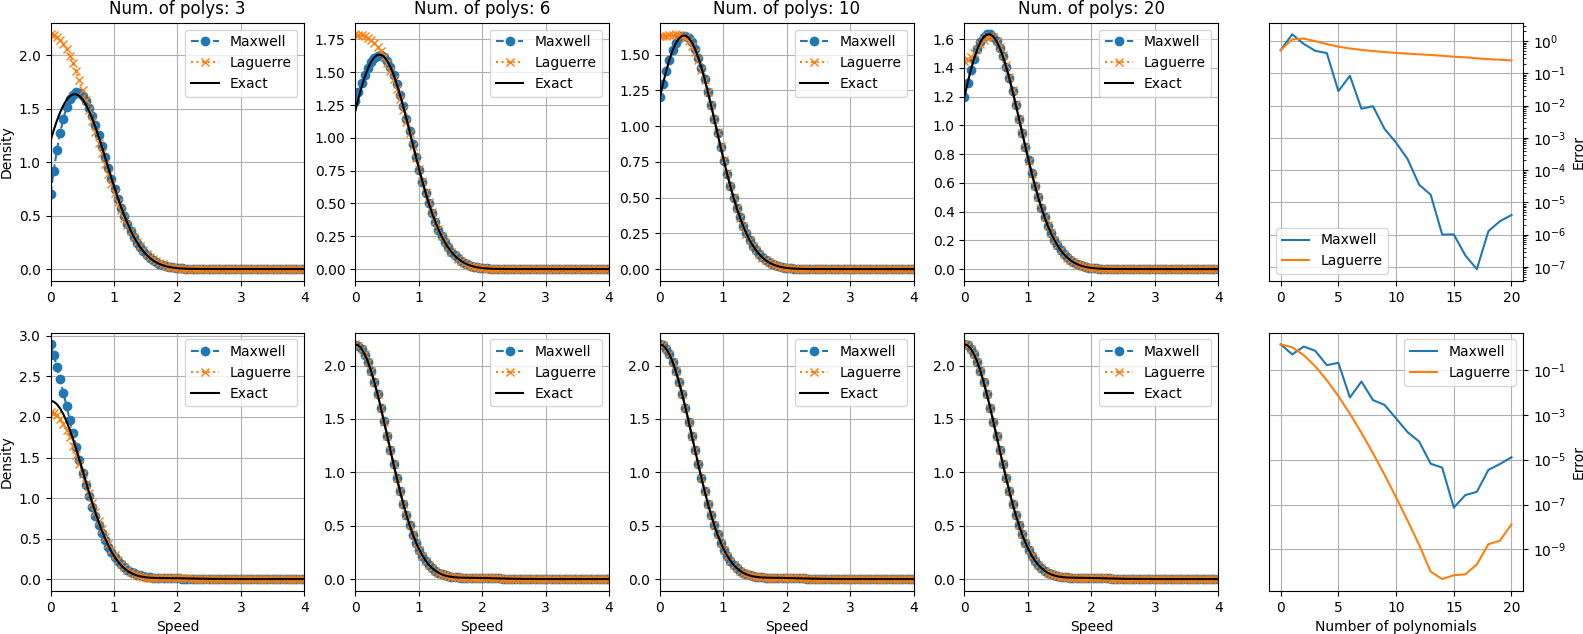
\includegraphics[width=.99\textwidth]{plot/density_analytic.png}
\caption{Compare $f\of{v}$. Top: $f\of{v} = (1.2+\sin\of{v})e^{-v^2}$, bottom: $f\of{v} = (1.2+\cos\of{v})e^{-v^2}$}
\label{}
\end{figure}
\begin{figure}[!h]
\centering
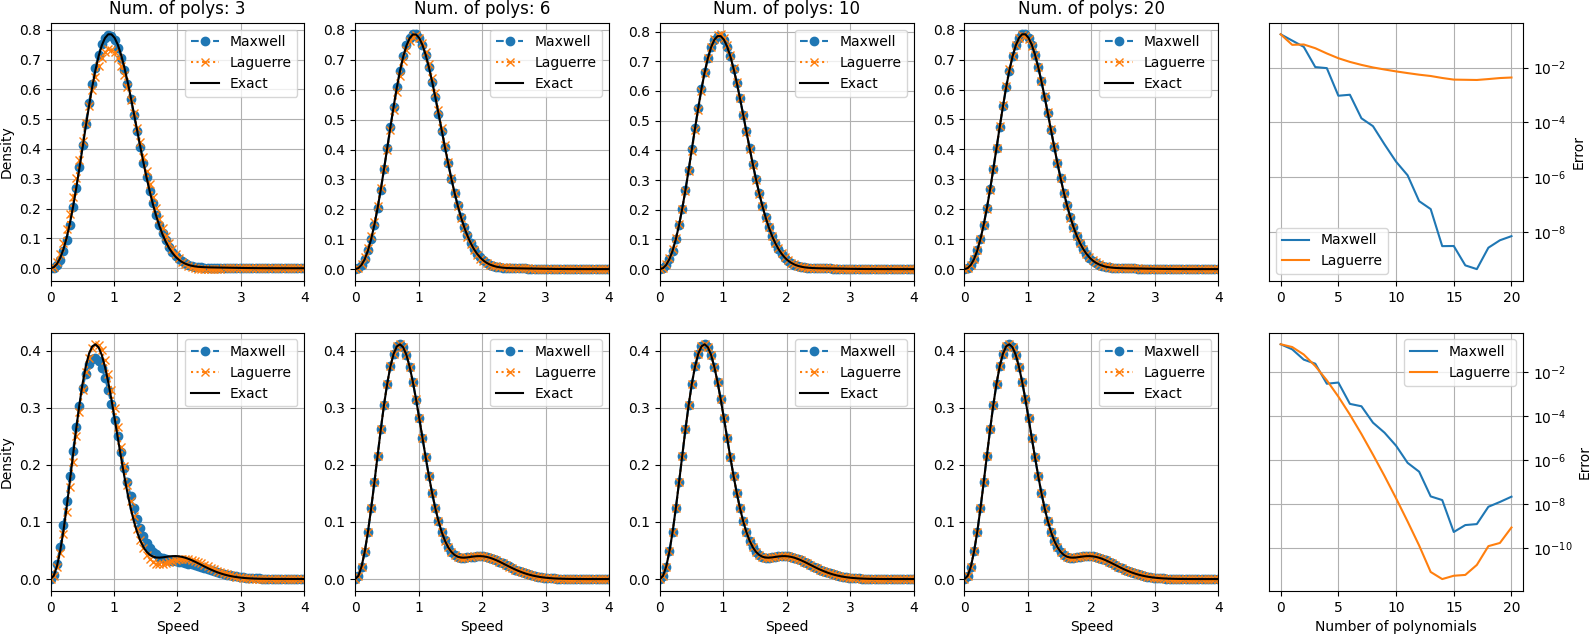
\includegraphics[width=.99\textwidth]{plot/speed_analytic.png}
\caption{Compare $f\of{v} v^2$. Top: $f\of{v} = (1.2+\sin\of{v})e^{-v^2}$, bottom: $f\of{v} = (1.2+\cos\of{v})e^{-v^2}$}
\label{}
\end{figure}

\begin{figure}[!h]
\centering
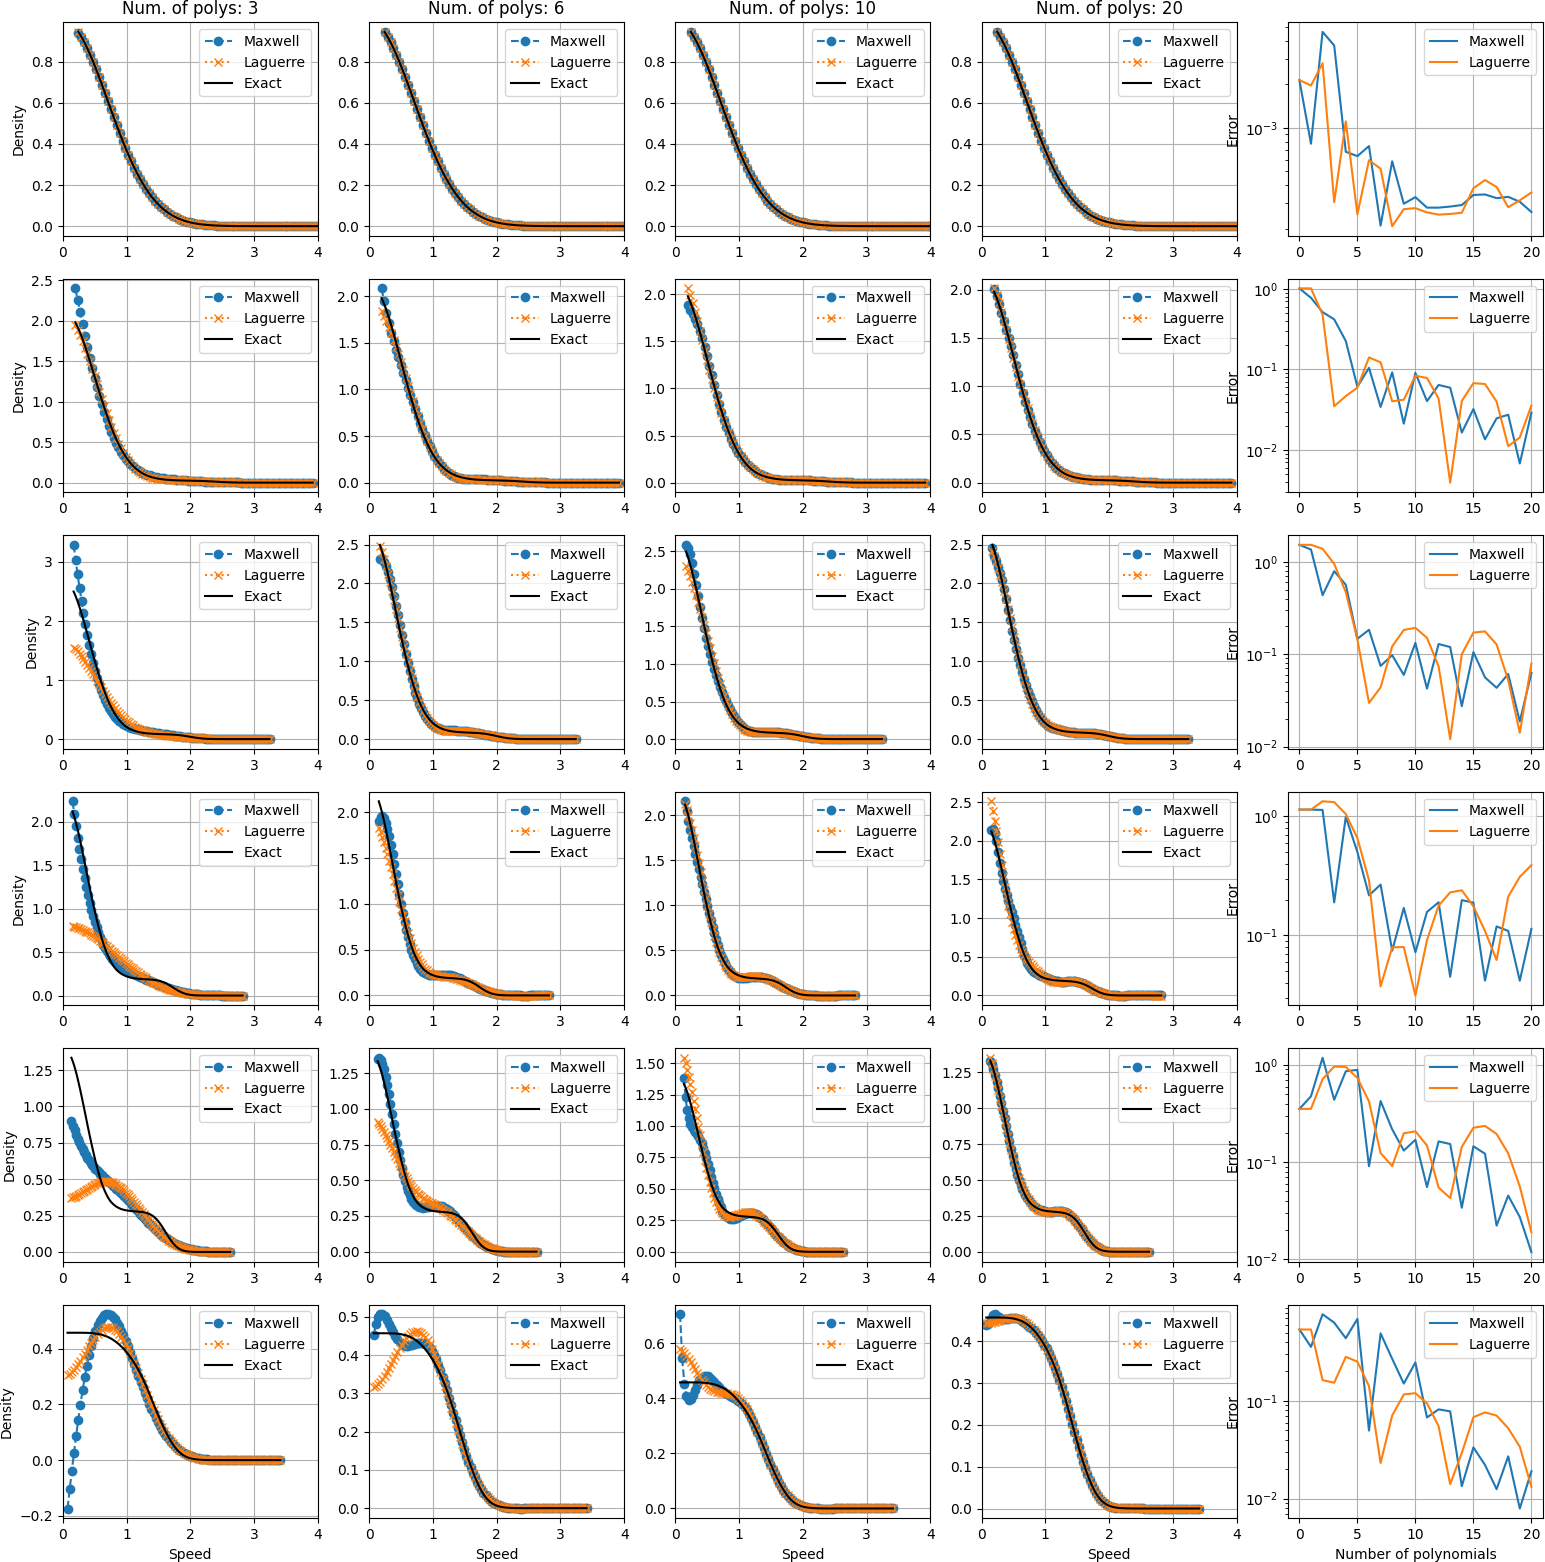
\includegraphics[width=.99\textwidth]{plot/density_bolsig.png}
\caption{Compare $f\of{v}$.}
\label{}
\end{figure}
\begin{figure}[!h]
\centering
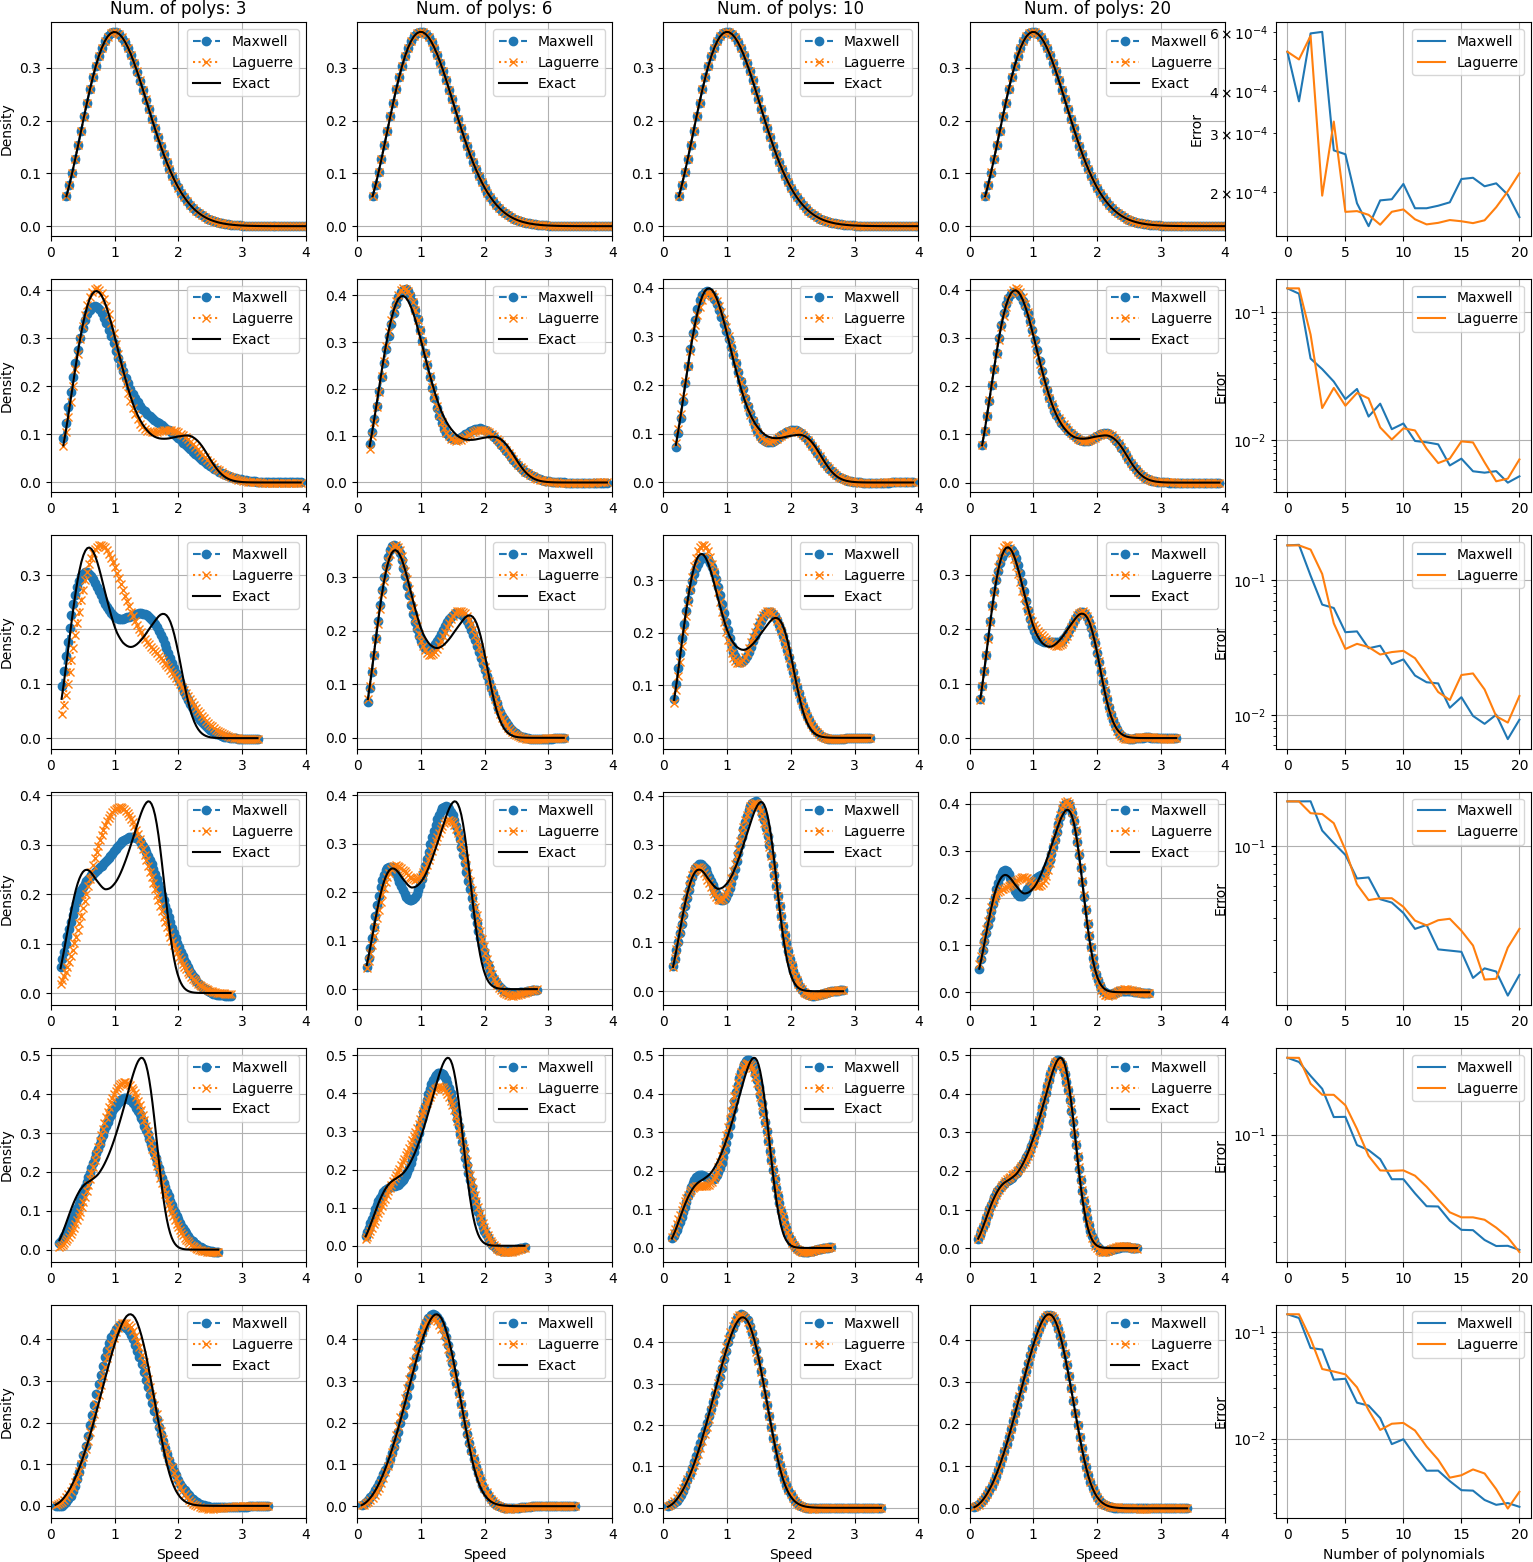
\includegraphics[width=.99\textwidth]{plot/speed_bolsig.png}
\caption{Compare $f\of{v} v^2$.}
\label{}
\end{figure}


\end{document}